\documentclass[english,notitlepage]{article}  % defines the basic parameters of the document
\usepackage[T1]{fontenc} %for å bruke æøå
\usepackage[utf8]{inputenc}
\usepackage{graphicx} %for å inkludere grafikk
\usepackage{mathpazo}
\usepackage[norsk]{babel}
% Standard stuff
\usepackage{amsmath,graphicx,varioref,verbatim,amsfonts,geometry,gensymb, multirow}
% colors in text
\usepackage[usenames,dvipsnames,svgnames,table]{xcolor}
% Hyper refs
\usepackage[colorlinks=true,allcolors=black]{hyperref}

\usepackage{caption}
\usepackage{enumitem}
\usepackage{tikz}             % draw figures manually
\usepackage{subfigure}        % imports a lot of cool and useful figure commands
\usepackage{float}
\usepackage{circuitikz}
\usepackage{listings}

\usepackage{csquotes}
\usepackage[backend=biber,style=alphabetic,sorting=ynt]{biblatex} %Imports biblatex package
\addbibresource{referanser.bib}

\begin{document}

\title{FYS3150\\Project 1}
\author{Brage Andreas Trefjord,\\Sigurd Sønvisen Vargdal,\\Nils Enric Canut Taugbøl,\\Frida Oleivsgard Sørensen}
\maketitle

\textit{GitHub repository:} \texttt{\url{https://github.com/NilsECT/FYS3150/tree/main/Project_1/Code}}

\section*{Problem 1}

  The one-dimensional Poisson equation can be written as

  \begin{equation}
    -\frac{d^2 u}{dx^2} = f(x) \label{eqn:poisson}
  \end{equation}

  where $f(x)$, the source term, is known. We assume a setup such that the source term is $f(x) = 100e^{-10x}$, $x \in [0, 1]$, and the boundary conditions are $u(0) = 0$ and $u(1)=0$.


  We want to check analytically that an exact solution to \hyperref[eqn:poisson]{equation \ref*{eqn:poisson}} can be given by

  \begin{equation}
    u(x) = 1 - (1-e^{-10})x - e^{-10x} \label{eqn:u(x)}
  \end{equation}

  We differentiate $u(x)$ twice and find that

  \begin{equation}
    \begin{split}
      \frac{d^2}{dx^2} u(x) &= \bigg( 1 - (1-e^{-10} ) x - e^{-10x} \bigg) \\
      &=  \frac{d}{dx} \bigg( 1-e^{-10} + 10 e^{-10x} \bigg) \\
      &=  - 100 e^{-10x} \\
      &= -f(x) \\
    \end{split}
  \end{equation}

  as we wanted. In addition, we check whether the boundary conditions are fulfilled:

  \begin{equation}
    \begin{split}
      u(0) &= \big( 1 - e^0 \big) = 1-1 \\
      &= 0 \\
      u(1) &= 1-1+e^{-10} - e^{-10} \\
      &= 0 \\
    \end{split}
  \end{equation}

  This means $u(x)$ in \hyperref[eqn:u(x)]{equation \ref*{eqn:u(x)}}
   is a solution to our specific setup.

\section*{Problem 2}

See code in the repository. You can see the resulting plot in \hyperref[fig:problem2]{figure
\ref*{fig:problem2}}.

\begin{figure}[H]
  \centering
  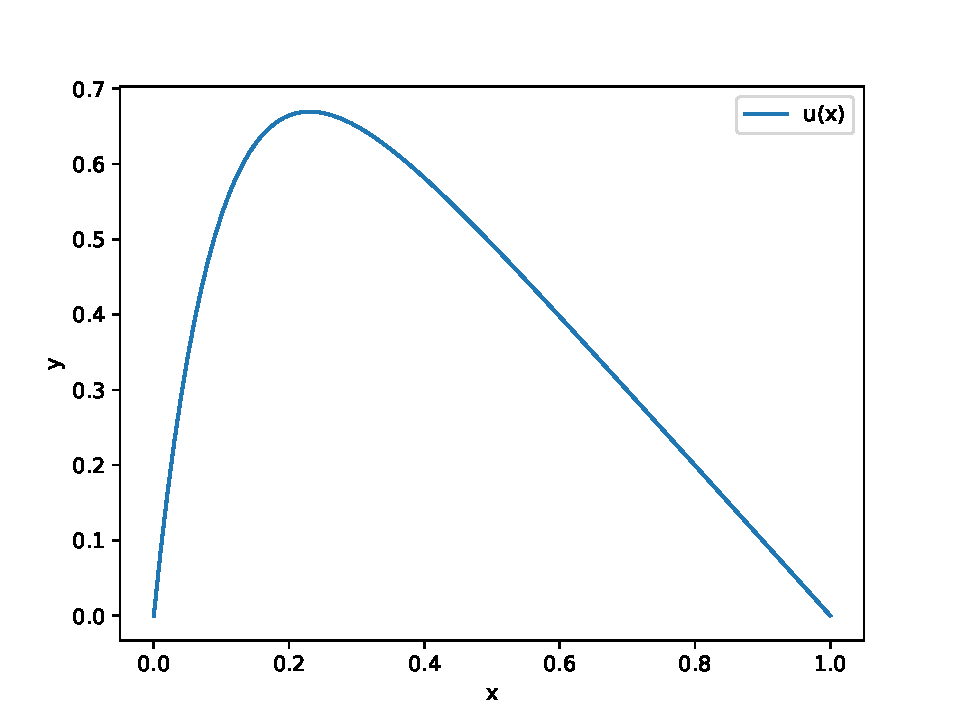
\includegraphics[width=0.6\linewidth]{../Code/Problem_2_plot.pdf}
  \caption{This is a plot of the exact solution to our differential equation.}
  \label{fig:problem2}
\end{figure}


\section*{Problem 3: Deriving the discretized Poisson equation.}

    Let's start by deriving the discretized version of $\frac{d^2u}{dx^2}$. First,
    we taylor expand the function $u(x+h)$ around the point $x$. We get:

    \begin{align*}
        u(x+h) &= \sum_{n=0}^{\infty} \frac{u^{(n)}(x)}{n!} h^n
        \\
        u(x+h) &= u(x) + u'(x) h + \frac{1}{2} u''(x) h^2 + \frac{1}{6} u'''(x) h^3 + O_1(h^4)
    \end{align*}

    where $O_1(h^2)$ is the remainder of the expansion, and $O(h) \equiv
    \frac{O_1(h^2)}{h}$. Now let's also Taylor expand $u(x-h)$ (again, around the
    point $x$).

    \begin{align*}
        u(x-h) &= \sum_{n=0}^{\infty} \frac{u^{(n)}(x)}{n!} (-h)^n
        \\
        u(x-h) &= u(x) - u'(x) h + \frac{1}{2} u''(x) h^2 - \frac{1}{6} u'''(x) h^3 + O_2(h^4)
    \end{align*}

    If we now add these two expansions together, we get:

    \begin{align*}
        u(x+h) + u(x-h) &= u(x) + u'(x) h + \frac{1}{2} u''(x) h^2 + \frac{1}{6} u'''(x) h^3
        + O_1(h^4)
        \\ & \hspace*{30pt} + u(x) - u'(x) h + \frac{1}{2} u''(x) h^2 - \frac{1}{6} u'''(x) h^3 + O_2(h^4)
        \\
        u(x+h) + u(x-h) &= 2u(x) + u''(x) h^2 + O_1(h^4) + O_2(h^4)
        \\
        u''(x) &= \frac{u(x+h) - 2u(x) + u(x-h)}{h^2} - \frac{O_1(h^4) + O_2(h^4)}{h^2}
        \\
        u''(x) &= \frac{u(x+h) - 2u(x) + u(x-h)}{h^2} + O(h^2)
    \end{align*}

    This can be discretized by letting $v_i \approx u(x)$, $v_{i+1} \approx u(x+h)$
    and $v_{i-1} \approx u(x-h)$. Since this is an approximation we can ignore the
    remainder, and our result becomes

    \begin{equation*}
        v''_i = \frac{v_{i+1} - 2v_i + v_{i-1}}{h^2}
    \end{equation*}

    Here $x$ is discretized as $i h$, where $h$ is the step length, and $i$ is the
    number of steps to reach the $x$ value. Using this, the discretization of the
    forcing term $f(x) = 100 e^{-10 x}$ becomes $f_i = 100 e^{-10 ih}$. Using this
    together with the discretized version of $v''(x)$ we get the complete
    discretized Poisson equation:

    \begin{equation}
        -\frac{v_{i+1} - 2v_i + v_{i-1}}{h^2} = 100 e^{-10 i h}
    \end{equation}

\section*{Problem 4}

    We have the following discretized expression:

    \begin{equation}\label{eq:second_derr}
        \left[\frac{u_{i+1} - 2u_i + u_{i-1}}{h^2} + O(h^2) = f_i\right]
    \end{equation}

    and we define $v_i = \frac{u_{i+1} - 2u_i + u_{i-1}}{h^2} \approx f_i$ and $\vec{v}$ to be the vector containing all $v_i$.

    With this in mind we can set up a matrix equation with a tri-diagonal matrix, $\boldsymbol{A}\vec{v} = \vec{g}$, as
    \begin{equation}\label{eq:mat_Avg}
        \begin{bmatrix}
            2 & -1 & 0 & 0 \\
            -1 & 2 & -1 & 0 \\
            0 & -1 & 2 & -1 \\
            0 & 0 & -1 & 2
        \end{bmatrix} \begin{bmatrix}
            v_1\\
            v_2\\
            v_3\\
            v_4
        \end{bmatrix} = \begin{bmatrix}
            g_1\\
            g_2\\
            g_3\\
            g_4
        \end{bmatrix}
    \end{equation}

    We can now compute $\boldsymbol{A}\vec{v}$ and compare each row to \hyperref[eq:second_derr]{equation \ref*{eq:second_derr}}. We can multiply \hyperref[eq:second_derr]{equation \ref*{eq:second_derr}} by $h^2$ on both sides and define the right-hand side to be $g_i$. Defining $\vec{g}$ appropriately we get the following:

    \begin{equation}\label{eq:mat_Vhf}
        \begin{bmatrix}
            2v_1 & -v_2 & 0 & 0 \\
            -v_1 & 2v_2 & -v_3 & 0 \\
            0 & -v_2 & 2v_3 & -v_4 \\
            0 & 0 & -v_3 & 2v_4
        \end{bmatrix} = \begin{bmatrix}
            g_1 \equiv h^2 f_1\\
            g_2 \equiv h^2 f_2\\
            g_3 \equiv h^2 f_3\\
            g_4 \equiv h^2 f_4
        \end{bmatrix}
    \end{equation}

    So we can represent the discretized equation of the second derrivative as a matrix equation.

\section*{Problem 5}

  We let $\vec{v}^* = [v^*_1, v^*_2, ... v^*_m]$ denote the vector of length $m$ that represents the complete solution of the discretized Poisson equation. The corresponding $x$ values are contained in $\vec{x} = [x_1, x_2, ..., x_m]$, with length $m$. We let \textbf{A} be an $n \times n$ matrix.

  \subsection*{Finding the relation between lengths $m$ and $n$}

    Writing out our matrix equation $\boldsymbol{A} \vec{v} = \vec{g}$, we get

    \begin{equation}
      \begin{bmatrix}
          2 & -1 & 0 & ... & 0 \\
          -1 & 2 & ... & ... & ... \\
          0 & ... & ... & -1 & 0 \\
          ... & ... & -1 & 2 & -1 \\
          0 & ... & 0 & -1 & 2 \\
      \end{bmatrix} \begin{bmatrix}
          v_1 \\
          v_2 \\
          ... \\
          v_{n-1} \\
          v_n \\
      \end{bmatrix} =
      \begin{bmatrix}
          g_1 \\
          g_2 \\
          ... \\
          g_{n-1} \\
          g_n \\
      \end{bmatrix}
    \end{equation}

    Further, by writing out the multiplication for the first element, we get

    \begin{equation}
      2 v_1 - v_2 = g_1  \label{eqn:v_0}
    \end{equation}

    But we see, from the discretized version of the Poisson equation in \hyperref[eq:mat_Vhf]{equation \ref*{eq:mat_Vhf}} that $v_1$ corresponds to the \emph{second} term in our solution $\vec{v}^*$, meaning the first element \emph{after} the boundary term (which in our case is $u(0) = v^*_1 = 0$). Including the boundary term, we get $2 v_1 - v_2 = -v_{0} + 2 v_1 - v_2 = g_1 $.

    Further, we write out the last element of the matrix equation:

    \begin{equation}
      -v_{n-1} + 2 v_n = g_n \label{eqn:v_n}
    \end{equation}

    Once again, we see that $v_n$ corresponds to the second-to-last element of $v^*$ (meaning the $v^*_{m-1})$, and the equation holds because the $m$th entry of $\vec{v}^*$ is $v^*_m = 0 = u(1)$.

    %If we denote the boundary term by $v_0^*$, then we have the correspondence $v_0 \rightleftarrow v^*_1$. Similarly, $g_0 \rightleftarrow f_1$.

    In general, we find there is a correspondence $v_i \longleftrightarrow v^*_{i+1}$ for $i \in \{1, ..., n\}$.

    As $\vec{v}$ has length $n$ and $\vec{v}^*$ has length $m$, we must have that $m = n+2$, where the additional two terms are due to the boundary terms.


  \subsection*{Which part of the complete solution do we get?}

    As $m = n+2$, we see that $\vec{v}$ only contains the 'middle' part of $\vec{v}^*$, meaning all elements excluding the two boundary terms.

    For the right hand side, we have to remember that $g_i$ corresponds to $f(x_{i+1})$.

\section*{Problem 6}

    The general expression for $\boldsymbol{A}\vec{v} = \vec{g}$ with $\vec{a}$, $\vec{b}$ and $\vec{c}$ being the sub-, main- and supdiagonal respectively is:
    \begin{equation}\label{eq:mat_Avg}
        \begin{bmatrix}
            b_1 & c_2 & 0 & 0 \\
            a_1 & b_2 & c_3 & 0 \\
            0 & a_2 & b_3 & c_4 \\
            0 & 0 & a_3 & b_4
        \end{bmatrix} \begin{bmatrix}
            v_1\\
            v_2\\
            v_3\\
            v_4
        \end{bmatrix} = \begin{bmatrix}
            g_1\\
            g_2\\
            g_3\\
            g_4
        \end{bmatrix}
    \end{equation}

    We can solve this with Gaussian elimination in two general steps: \hyperref[sec:forward]{[1]} Forward substitution and \hyperref[sec:backward]{[2]} Backward substitution.

    \subsection*{Forward substitution}\label{sec:forward}

    The goal here is to get an upper triangular matrix, that is we want to do the follwoing:
    \begin{equation*}
        \begin{bmatrix}
            \cdot & \cdot & \cdot & \cdot \\
            \cdot & \cdot & \cdot & \cdot \\
            \cdot & \cdot & \cdot & \cdot \\
            \cdot & \cdot & \cdot & \cdot
        \end{bmatrix} \begin{bmatrix}
            \cdot\\
            \cdot\\
            \cdot\\
            \cdot
        \end{bmatrix} = \begin{bmatrix}
            \cdot\\
            \cdot\\
            \cdot\\
            \cdot
        \end{bmatrix}
        \rightarrow
        \begin{bmatrix}
            \cdot & \cdot & \cdot & \cdot \\
            0 & \cdot & \cdot & \cdot \\
            0 & 0 & \cdot & \cdot \\
            0 & 0 & 0 & \cdot
        \end{bmatrix} \begin{bmatrix}
            \cdot\\
            \cdot\\
            \cdot\\
            \cdot
        \end{bmatrix} = \begin{bmatrix}
            \cdot\\
            \cdot\\
            \cdot\\
            \cdot
        \end{bmatrix}
    \end{equation*}

    So we want to get rid of all $a_i$ entries in \hyperref[eq:mat_Avg]{the matrix equation (\ref*{eq:mat_Avg})}. We will number and denote the rows with roman numerals.

    \begin{gather}
        \RN{2} = \RN{2} - \frac{a_2}{b_1}\RN{1}\\
        \text{The diagonal new entries will be denoted } \tilde{b_i} \nonumber \\
        \RN{3} = \RN{3} - \frac{a_3}{\tilde{b_2}}\RN{2}\\
        \RN{4} = \RN{4} - \frac{a_4}{\tilde{b_3}}\RN{3}\\
    \end{gather}

    This gives us the following algorithm for precdure
    \begin{gather}\label{eq:for}
        \tilde{b_1} = b_1 \\
        \tilde{b_i} = b_i - \frac{a_i}{\tilde{b_{i-1}}}c_{i-1}\\\label{line:for_b}
        \tilde{g_1} = g_1 \\
        \tilde{g_i} = g_i - \frac{a_i}{\tilde{b_{i-1}}}\tilde{g_{i-1}}\\\label{line:for_g}
    \end{gather}
    This will be for $i = 2, 3, ..., n$ for a general tridiagonal matrix.

  \subsection*{Backward substitution}\label{sec:backward}

    Now that we have done the forward substitution we want to find the solution to all $v_i$ from the following equation:

    \begin{equation}
        \begin{bmatrix}
            \tilde{b_1} & c_2 & 0 & 0 \\
            0 & \tilde{b_2} & c_3 & 0 \\
            0 & 0 & \tilde{b_3} & c_4 \\
            0 & 0 & 0 & \tilde{b_4}
        \end{bmatrix} \begin{bmatrix}
            v_1\\
            v_2\\
            v_3\\
            v_4
        \end{bmatrix} = \begin{bmatrix}
            \tilde{g_1}\\
            \tilde{g_2}\\
            \tilde{g_3}\\
            \tilde{g_4}
        \end{bmatrix}
    \end{equation}

    we quickly see that $v_4 = \frac{\tilde{g_4}}{\tilde{b_4}}$ and to get the remaining $v_i$ we move up with the following algorithm (we include the case of $v_n$ to generalize the algorithm):
    \begin{gather}\label{eq:back}
        v_n = \frac{\tilde{g_n}}{\tilde{b_n}}\\
        v_i = \frac{\tilde{g_i} - c_iv_{i-1}}{\tilde{b_i}}\\
    \end{gather}
    for $i = n-1, n-2, ..., 2, 1$.

  \subsection*{FLOPs}

    We can see that \hyperref[eq:for]{algorithm \ref*{eq:for}} requires $2(n-1)$ floating point operations. $n-1$ FLOPs for \hyperref[line:for_b]{equation (\ref*{line:for_b})} and \hyperref[line:for_g]{equation (\ref*{line:for_g})} each. From \hyperref[eq:back]{equation \ref*{eq:back}} we can count $3(n-1) + 1$ FLOPs. This gives us a total of $5n - 4$ FLOPs to solve $\boldsymbol{A}\vec{v} = \vec{g}$ with a tridiagonal matrix of dimentions $n\times n$.

\section*{Problem 7}

See code in repository. The result is in \hyperref[fig:problem7]{figure \ref*{fig:problem7}}.

\begin{figure}[H]
  \centering
  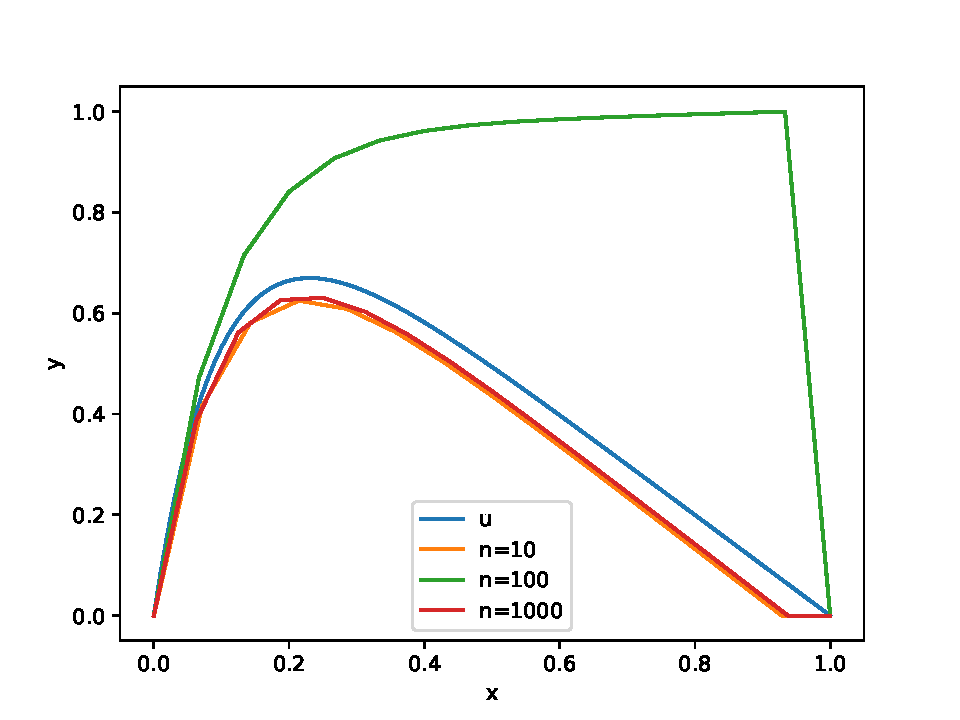
\includegraphics[width=0.6\linewidth]{../Code/Problem_7_plot.pdf}
  \caption{Plot of the solution to problem 7.}
  \label{fig:problem7}
\end{figure}

\section*{Problem 8}

See code in repository. The result for a), b) and c), is shown in
\hyperref[fig:problem8a]{figure \ref*{fig:problem8a}},
\hyperref[fig:problem8b]{figure \ref*{fig:problem8b}} and
\hyperref[fig:problem8c]{figure \ref*{fig:problem8c}} respectively.

\begin{figure}[H]
  \centering
  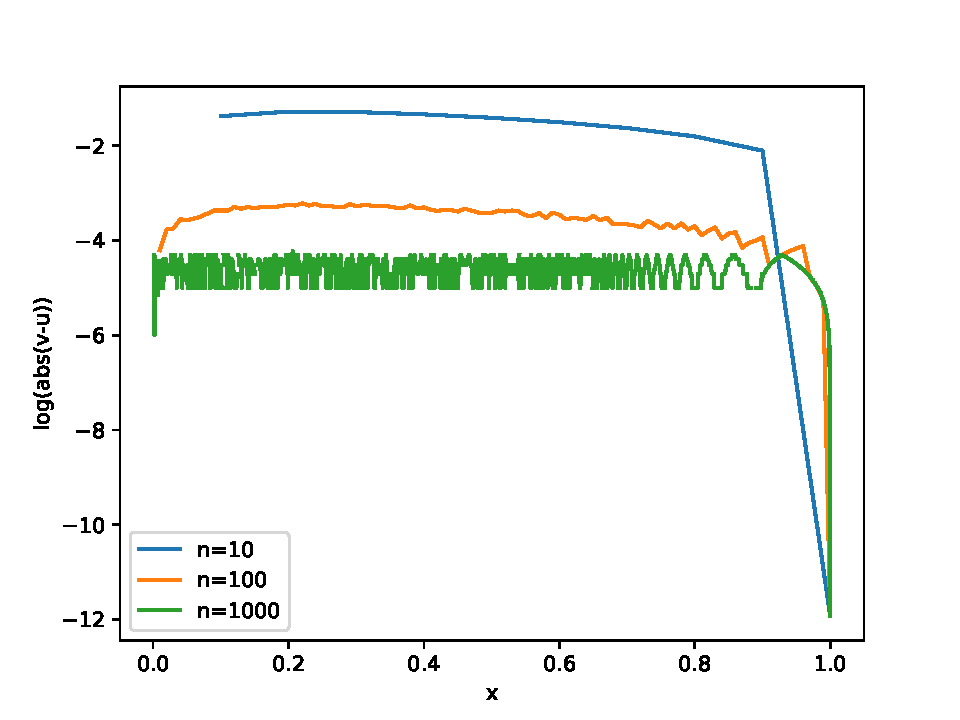
\includegraphics[width=0.6\linewidth]{../Code/log10_abs_err.pdf}
  \caption{Plot of the solution to problem 8a).}
  \label{fig:problem8a}
\end{figure}

\begin{figure}[H]
  \centering
  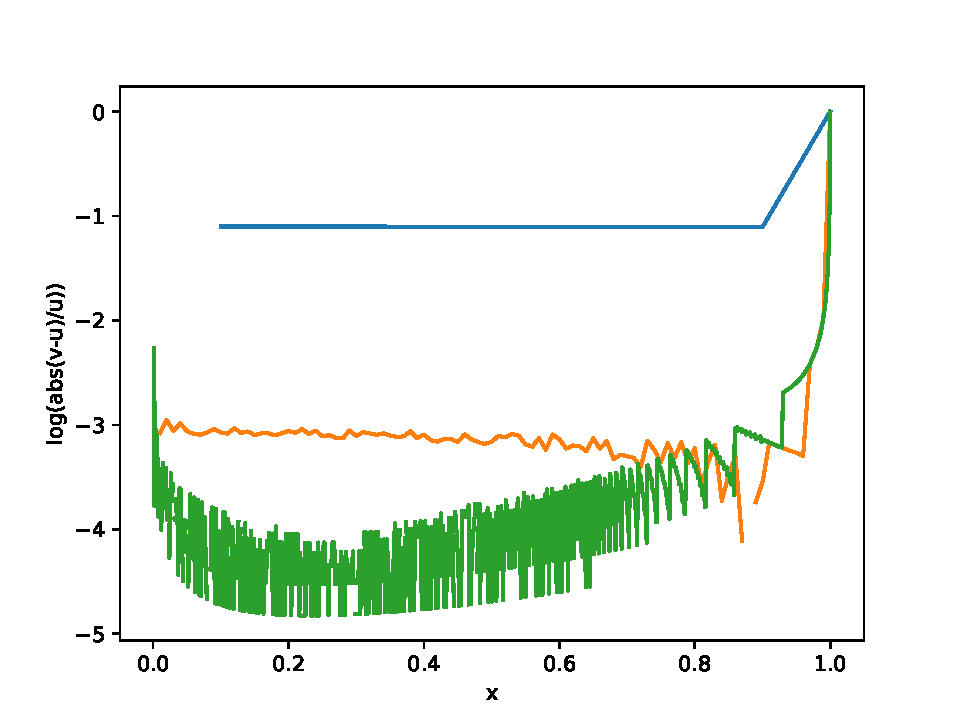
\includegraphics[width=0.6\linewidth]{../Code/log10_rel_err.pdf}
  \caption{Plot of the solution to problem 8b).}
  \label{fig:problem8b}
\end{figure}

\begin{figure}[H]
  \centering
  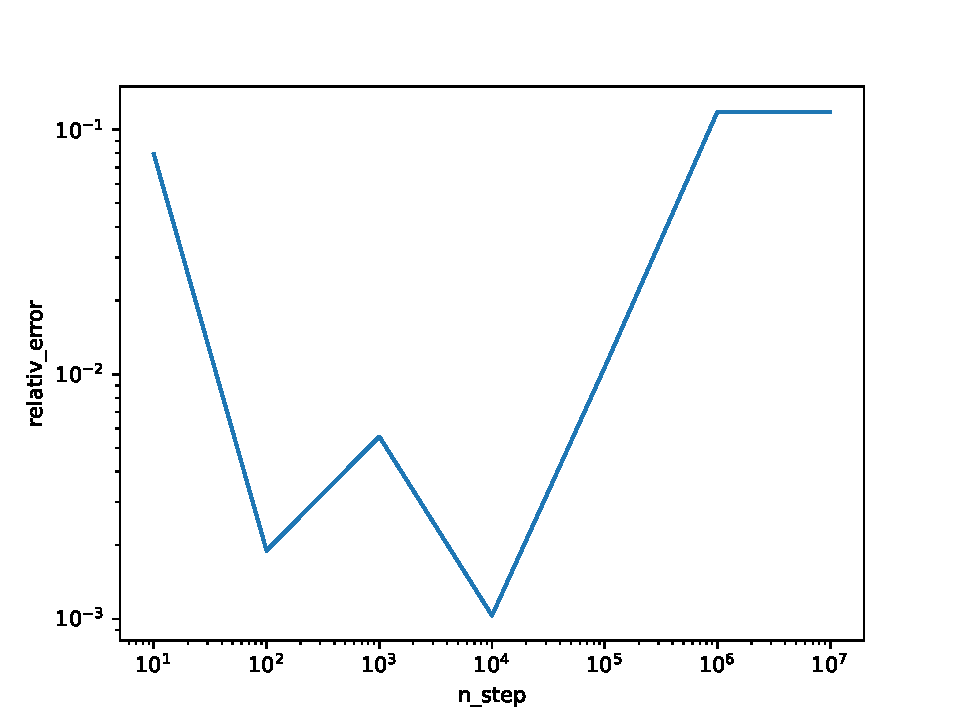
\includegraphics[width=0.6\linewidth]{../Code/Problem_8_c_plot.pdf}
  \caption{Plot of the solution to problem 8c).}
  \label{fig:problem8c}
\end{figure}

We see that we start off with a larger error, which then decreases when we
increase the number of steps. This makes sense, because the truncation error
gets smaller when $n_{steps}$ is large. After $n_{steps} = 10^4$ the maximum
relative error increases. This is because the round-off error when computing
numerically increases when we have to deal with small numbers. When $n_{steps}$
becomes large, each step-length becomes smaller, and our computers can't
represent these numbers well enough.

\section*{Problem 9}

  \subsection*{Specialize the algorithm}


    We want to specialize the algorithm from Problem 6 for the special case where $\boldsymbol{A}$ is specified by the signature $(-1, 2, -1)$. This menas that $\vec{a}$ and $\vec{c}$ are vectors of length $n-1$, consisting only of the value $-1$, and $\vec{b}$ is an $n$-length vector filled with the value $2$.

    Substituting every $a_i, c_i$ with $-1$ and $b_i$ with $2$, we obtain the following equations for

    \begin{equation}
      \begin{split}
        \tilde{b}_1 &= b_1 = 2 \\
        \tilde{b}_i &= b_i - \frac{a_i}{\tilde{b}_{i-1}} c_{i-1} = 2 - \frac{1}{\tilde{b}_{i-1}} \\ \label{eqn:specalg_b}
       \end{split}
    \end{equation}

    \begin{equation}
      \begin{split}
        \tilde{g}_1 &= g_1 \\
        \tilde{g}_i &= g_i - \frac{a_i}{\tilde{b}_{i-1}} \tilde{g}_{i-1} = g_i + \frac{\tilde{g}_{i-1}}{\tilde{b}_{i-1}} \\ \label{eqn:specalg_g}
       \end{split}
    \end{equation}

    Similarly, for the backward substitution we get the following equations:

    \begin{equation}
      \begin{split}
        v_n &= \frac{\tilde{g}_n}{\tilde{b_n}} \\
        v_i &= \frac{\tilde{g}_i - c_i v_{i+1}}{\tilde{b}_i} = \frac{\tilde{g}_i + v_{i+1}}{\tilde{b}_i} \\ \label{eqn:specalg_v}
       \end{split}
    \end{equation}

  \subsection*{Number of FLOPs in specialized algorithm}

    We count the number of FLOPs required for the special algorithm.

    When calculating every element of $\vec{\tilde{b}}$, we see from \hyperref[eqn:specalg_b]{equation \ref*{eqn:specalg_b}}  that we perform 2 FLOPs (consisting of addition and division) for every $i \in [1, N-1]$. The initial element $b_1$ requires no FLOPs. Exactly the same holds for calculating $\vec{\tilde{g}}$ in \hyperref[eqn:specalg_g]{equation \ref*{eqn:specalg_g}}.

    However, for the backward substitution in \hyperref[eqn:specalg_v]{equation \ref*{eqn:specalg_v}}, we see that in addition to the $2(n-1)$ FLOPs, we need one more for the last term $v_n$.

    In total, we require

    \begin{equation}
      3 ~ \cdotp \big[ 2(n-1)\big] + 1 = 6n-5 \text{ FLOPs}
    \end{equation}

    \subsection*{Implement algorithm in code}

    Lastly, we write code that implements the algorithm. See code in repository.

\section*{Problem 10}
    
\begin{figure}[H]
  \begin{center}
    \includegraphics*[width=\linewidth]{../Code/plot_P10.pdf}
    \caption{Logarithmic plot of the time each algorithm takes to compute the same equations with increasing number of steps. We see that the algorithms show a diverging tendency with an increasing number of steps.}
    \label{fig:P10}
  \end{center}
\end{figure}

We've run each algorithm 100 times for each number of steps growing exponentially from 10 to $10^6$. The plot in figure \hyperref[fig:P10]{figure \ref*{fig:P10}} shows the different times each algorithm takes with the standard errors of each mean. We can see that for greater and greater number of steps, the special algorithm proves more and more efficient.

\end{document}
